
%使用XeLaTeX编译
%版权所有,翻版必究
%本文件由程序自动生成,任何修改将被覆盖
%2019 年 01 月 23 日




\FloatBarrier
\section{
QML语法
}\label{c000011s000000}


%编码
\FloatBarrier
\subsection{
文件编码
}\label{c000011s000000s03}


自从Qt 5开始,Qt所有源代码只接受一种编码,
那就是UTF\hspace{0.05em}\rule[0.7ex]{0.4em}{0.65pt}\hspace{0.05em}8。

无论是C{\sourcefonttwo{}+}{\sourcefonttwo{}+}、QML、JavaScript或者是qmake工程文件,
都应当只采用UTF\hspace{0.05em}\rule[0.7ex]{0.4em}{0.65pt}\hspace{0.05em}8编码。

特别的是,有些UTF\hspace{0.05em}\rule[0.7ex]{0.4em}{0.65pt}\hspace{0.05em}8文件开头会有三个特殊字符:
\begin{littlelongworld}0xEF0xBB0xBF
\end{littlelongworld}以以上三个特殊字符开头的UTF\hspace{0.05em}\rule[0.7ex]{0.4em}{0.65pt}\hspace{0.05em}8文件一般
被称为UTF\hspace{0.05em}\rule[0.7ex]{0.4em}{0.65pt}\hspace{0.05em}8 with BOM。

Qt集成开发环境所有编译器都识别BOM,除了qmake。

也就是读者在书写qmake工程文件(\raisebox{-0.35ex}{\sourcefonttwo{}*}.pro或者\raisebox{-0.35ex}{\sourcefonttwo{}*}.pri文件)时
一定不能给文件添加BOM。实际上,qmake只识别ASCII码的
127个字符。不应当在qmake工程文件中使用超出ASCII码的
字符。

但是在书写C{\sourcefonttwo{}+}{\sourcefonttwo{}+}、QML、JavaScript文件时,可以给文件添加BOM。

在不同的操作系统下,系统的默认文件编码会有所不同。
由于历史原因和编程习惯,一些计算机语言不要求在源码中指定源码的
编码。
这就会造成,如果不给这些计算机语言的源码添加BOM,
编译器会错误的识别源代码编码,
造成编译错误和运行逻辑错误。

对于这类计算机语言,最好对它们的源码添加BOM。

而对于一些现代计算机语言比如Html,
一般的在源码中就指定了源码的编码。
因而,对于这些计算机语言,最好不要对它们的源码添加BOM。

本书对C{\sourcefonttwo{}+}{\sourcefonttwo{}+}源文件,QML源文件,以及JavaScript源文件添加BOM
以最大程度降低平台差异性。

%注释与帮助
\FloatBarrier
\subsection{
注释与帮助
}\label{c000011s000000s02}


C{\sourcefonttwo{}+}{\sourcefonttwo{}+}、QML以及JavaScript的注释语法都是一致的:

\begin{itemize}
\item //单行注释
\item /\raisebox{-0.35ex}{\sourcefonttwo{}*}多行注释\raisebox{-0.35ex}{\sourcefonttwo{}*}/
\end{itemize}

而qmake的工程文件只支持单行注释:
\begin{itemize}
\item {\sourcefonttwo\#}单行注释
\end{itemize}


%http://www.glimix.com/archives/1594
%https://wiki.qt.io/QDoc
%http://doc.qt.io/qt-5/qdoc-index.html

Qt集成开发环境自带一个工具可以
自动提取C{\sourcefonttwo{}+}{\sourcefonttwo{}+}与QML中的注释并生成帮助
文件。

此工具被称为QDoc。

QDoc是一套庞大的体系,读者可以在QtCreator中输入
qdoc以获得更多帮助。
如\figurename\ \ref{p000043}。

%begin图片
\begin{figure}[htb] %浮动体 here and top ...
%there must use marginnote ...
\marginnote{\setlength\fboxsep{2pt}\fbox{\footnotesize{\kaishu\figurename\,}\footnotesize{\ref{p000043}}}}\centering %中心对齐
\setlength\fboxsep{0pt}\fcolorbox[rgb]{0,0,0}{0.97,0.98,0.99}{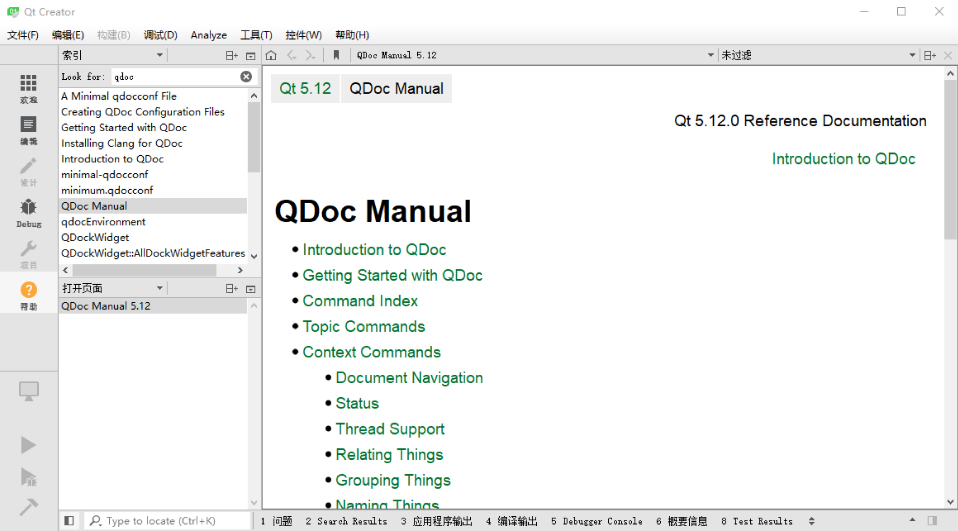
\includegraphics[width=0.95\textwidth]{the_book_image/p000043.pdf}} %图片路径
\caption{QDoc} %标题
\label{p000043} %索引
\end{figure}
%end图片






%使用XeLaTeX编译
%版权所有,翻版必究
%本文件由程序自动生成,任何修改将被覆盖
%2019 年 01 月 23 日




\FloatBarrier
\subsection{
类型与对象属性
}\label{c000011s000000s01}


QML被设计为一门可以支持JavaScript的
弱类型语言。

虽然绝大多数JavaScript代码可以在QML
环境之中正常运行。
但并不意味着JavaScript语义与QML语义
完全一致。

一般而言,QML对JavaScript做了适当扩展。

如果读者完全按照JavaScript语义理解
QML类型系统,倒也不算错。
但损失大量效率是免不了的。

QML类型可以分为
基本类型、
扩展类型
和用户自定义类型。

%QML Basic Types
%bool
%double
%enumeration
%int
%list
%real
%string
%url
%var
%date
%point
%rect
%size


%基本类型
\FloatBarrier
\subsubsection{
基本类型
}\label{c000011s000000s01s01}


%http://doc.qt.io/qt-5/qml-int.html

\tablename\ \ref{tb000005}展示了
QML中的基本类型。


%使用XeLaTeX编译
%版权所有,翻版必究
%本文件由程序自动生成,任何修改将被覆盖
%2019 年 01 月 23 日



%表
\begin{longtable}{ccc}

%表头....
\toprule{}类名 
&
分类
&
简介%there must use marginnote ...
\marginnote{\setlength\fboxsep{2pt}\fbox{\footnotesize{\kaishu\tablename\,}\footnotesize{\ref{tb000000}}}}
\\ \midrule 
\endfirsthead

%表尾...
\bottomrule
\caption{ThresholdMask}\label{tb000000} 
\endlastfoot

%重复表头
\toprule{}类名 
&
分类
&
简介
\\ \midrule
\endhead
%重复表尾
\midrule
\endfoot 
Blend & aabbc & cccc \\
BrightnessContrast & aabbc & cccc \\
ColorOverlay & aabbc & cccc \\
Colorize & aabbc & cccc \\
Desaturate & aabbc & cccc \\
GammaAdjust & aabbc & cccc \\
HueSaturation & aabbc & cccc \\
LevelAdjust & aabbc & cccc \\
ConicalGradient & aabbc & cccc \\
LinearGradient & aabbc & cccc \\
RadialGradient & aabbc & cccc \\
Displace & aabbc & cccc \\
DropShadow & aabbc & cccc \\
InnerShadow & aabbc & cccc \\
FastBlur & aabbc & cccc \\
GaussianBlur & aabbc & cccc \\
MaskedBlur & aabbc & cccc \\
RecursiveBlur & aabbc & cccc \\
DirectionalBlur & aabbc & cccc \\
RadialBlur & aabbc & cccc \\
ZoomBlur & aabbc & cccc \\
Glow & aabbc & cccc \\
RectangularGlow & aabbc & cccc \\
OpacityMask & aabbc & cccc \\
ThresholdMask  & aabbc & cccc \\
\end{longtable}
%表





%使用XeLaTeX编译
%版权所有,翻版必究
%本文件由程序自动生成,任何修改将被覆盖
%2019 年 01 月 23 日





\tablename\ \ref{tb000005}中的基本类型
是直接内嵌在QML引擎中的。
Qt并没有提供接口可以让读者直接定义
像int,double这样的原生
类型。读者如果需要扩展QML类型,只能继承自QObject类或其子类。


    % Data Type Conversion Between QML and C++


\begin{itemize}

\item bool

QML中的布尔类型根绝大多数计算机语言一致,只有true和false两个值。
\item int

QML中的整型对应于C{\sourcefonttwo{}+}{\sourcefonttwo{}+}中的int,其安全使用范围是
\hspace{0.05em}\rule[0.7ex]{0.4em}{0.65pt}\hspace{0.05em}2000000000\raisebox{0.16ex}{\sourcefonttwo\~{}}2000000000。

很多时候应用程序需要的是int64,这时候应当使用
var。

\item double与real

QML中的double与real没有什么区别,对应于
IEEE 754标准中规定的64位双精度浮点数。
\item enumeration

QML中的枚举类型,既可来源于C{\sourcefonttwo{}+}{\sourcefonttwo{}+}的导出,
也可来源于QML中的定义。
\item url

QML中的路径都是url类型,它与QUrl一致。
\item string

QML中的字符串除了可以使用JavaScript中的所有方法之外,
还可以使用QString中的arg函数。
\item list

QML中list被设计用于包装QML对象,如果需要基本类型容器,应当使用var。
\item var

QML中的var用于代表一切合法类型,包括信号槽,容器,基本类型以及一切
可以被QVariant识别的类型……

在一些时候读者会发现variant这个词,它与var是一致的。
支持这个词仅仅是为了兼容老版本的QML。

\end{itemize}

%扩展类型
\FloatBarrier
\subsubsection{
扩展类型
}\label{c000011s000000s01s02}

除了第\ref{c000011s000000s01s01}节提到的
基本类型之外,
不同的QML库还提供了一些扩展类型。

对于一般读者而言,这些扩展类型和基本类型之间除了构造方法之外
没有什么不同。


%自定义类型
\FloatBarrier
\subsubsection{
自定义类型
}\label{c000011s000000s01s03}

QML被设计为一门扩展Qt C{\sourcefonttwo{}+}{\sourcefonttwo{}+}的语言,
因而,从Qt C{\sourcefonttwo{}+}{\sourcefonttwo{}+}向QML导出自定义类是相当自然的。
详细内容见第\ref{c000012}章。

%QML常用基本与Qt C++常用类型对应表
\FloatBarrier
\subsubsection{
QML常用基本与Qt C{\sourcefonttwo{}+}{\sourcefonttwo{}+}常用类型对应表
}\label{c000011s000000s01s04}


\tablename\ \ref{tb000005}展示了
QML常用基本与Qt C{\sourcefonttwo{}+}{\sourcefonttwo{}+}常用类型的对应关系。


%使用XeLaTeX编译
%版权所有,翻版必究
%本文件由程序自动生成,任何修改将被覆盖
%2019 年 01 月 23 日



%表
\begin{longtable}{ccc}

%表头....
\toprule{}类名 
&
分类
&
简介%there must use marginnote ...
\marginnote{\setlength\fboxsep{2pt}\fbox{\footnotesize{\kaishu\tablename\,}\footnotesize{\ref{tb000000}}}}
\\ \midrule 
\endfirsthead

%表尾...
\bottomrule
\caption{ThresholdMask}\label{tb000000} 
\endlastfoot

%重复表头
\toprule{}类名 
&
分类
&
简介
\\ \midrule
\endhead
%重复表尾
\midrule
\endfoot 
Blend & aabbc & cccc \\
BrightnessContrast & aabbc & cccc \\
ColorOverlay & aabbc & cccc \\
Colorize & aabbc & cccc \\
Desaturate & aabbc & cccc \\
GammaAdjust & aabbc & cccc \\
HueSaturation & aabbc & cccc \\
LevelAdjust & aabbc & cccc \\
ConicalGradient & aabbc & cccc \\
LinearGradient & aabbc & cccc \\
RadialGradient & aabbc & cccc \\
Displace & aabbc & cccc \\
DropShadow & aabbc & cccc \\
InnerShadow & aabbc & cccc \\
FastBlur & aabbc & cccc \\
GaussianBlur & aabbc & cccc \\
MaskedBlur & aabbc & cccc \\
RecursiveBlur & aabbc & cccc \\
DirectionalBlur & aabbc & cccc \\
RadialBlur & aabbc & cccc \\
ZoomBlur & aabbc & cccc \\
Glow & aabbc & cccc \\
RectangularGlow & aabbc & cccc \\
OpacityMask & aabbc & cccc \\
ThresholdMask  & aabbc & cccc \\
\end{longtable}
%表





%使用XeLaTeX编译
%版权所有,翻版必究
%本文件由程序自动生成,任何修改将被覆盖
%2019 年 01 月 23 日





对于\tablename\ \ref{tb000005}中
没有提及的类型,一般用var代替即可。

%容器
\FloatBarrier
\subsubsection{
QML可以识别的Qt C{\sourcefonttwo{}+}{\sourcefonttwo{}+}容器
}\label{c000011s000000s01s05}


一般而言如果一个Qt C{\sourcefonttwo{}+}{\sourcefonttwo{}+}类型能够被QML识别,
那么用QList和QMap包装这个对象,也能够被QML识别。

比如,Qt C{\sourcefonttwo{}+}{\sourcefonttwo{}+}端
QUrl能够被
QML识别,那么
QList<QUrl>
也能被QML识别。

更加一般的是Qt C{\sourcefonttwo{}+}{\sourcefonttwo{}+}端的
QVariantList容器和QVariantMap容器,
总是能被QML端识别。
但比使用更加具体的对象容器效率要低。

除了可以使用QList和QMap
包装对象,也可以使用
QVector、
std::vector包装
对象。

值得注意的是,包装QString最好使用QStringList类,
包装QObject \raisebox{-0.35ex}{\sourcefonttwo{}*} 最好使用QObjectList类。


% ______all_key_words
% the_book_chapter the_book_subsection the_book_subsubsection
% the_book_section the_book_image the_book_table
% the_book_file the_book_tree_file the_book_command_file
% littlelongworld tabbing ref
% figurename tablename filesourcenumbernameone
% treeindexnumbernameone commandnumbernameone footnote
% item itemize comment textbullet
% \hspace*{\parindent}
% FloatBarrier







%使用XeLaTeX编译
%版权所有,翻版必究
%本文件由程序自动生成,任何修改将被覆盖
%2019 年 01 月 23 日








% ______all_key_words
% the_book_chapter the_book_subsection the_book_subsubsection
% the_book_section the_book_image the_book_table
% the_book_file the_book_tree_file the_book_command_file
% littlelongworld tabbing ref
% figurename tablename filesourcenumbernameone
% treeindexnumbernameone commandnumbernameone footnote
% item itemize comment textbullet
% \hspace*{\parindent}
% FloatBarrier







%使用XeLaTeX编译
%版权所有,翻版必究
%本文件由程序自动生成,任何修改将被覆盖
%2019 年 01 月 23 日



